 \section{Anhang}
    \begin{figure}[H]
        \centering
        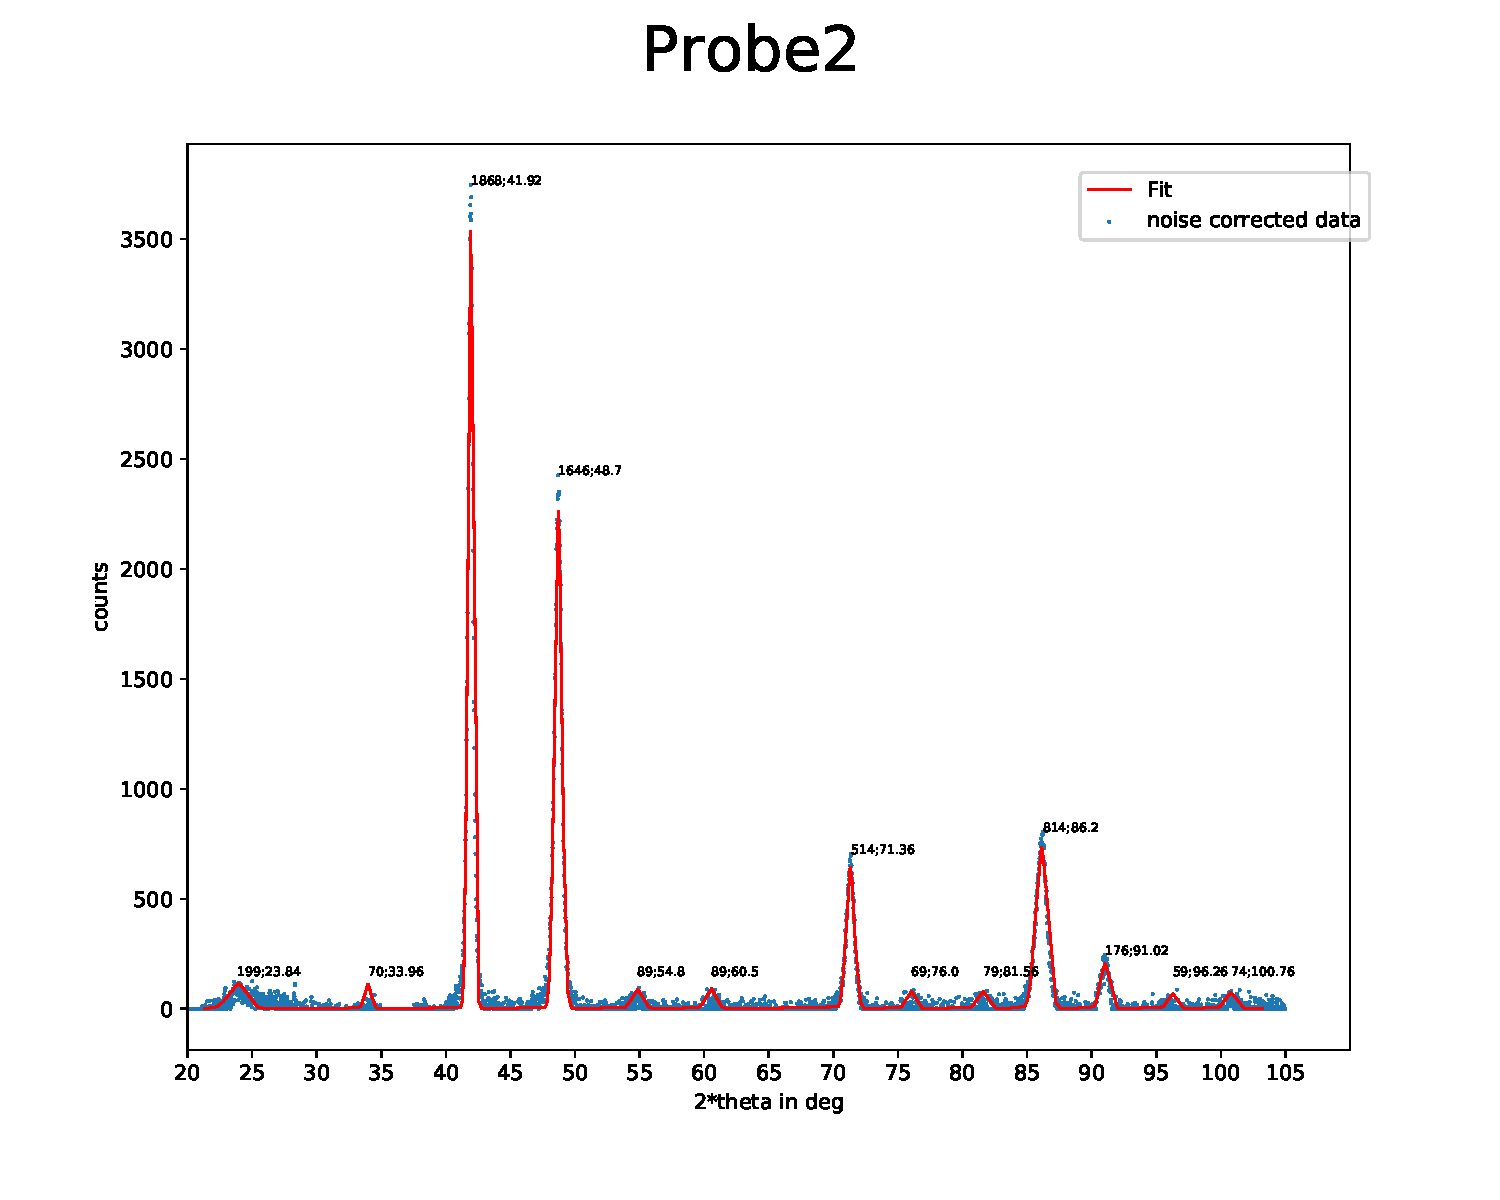
\includegraphics[width=0.8\textwidth]{Messdaten/Auswertungsskripte/Probe2.pdf}
        \caption{Röntgendiffraktogramm Probe 2}
        \label{Röntgendiffraktogramm Probe 2}
    \end{figure}

    \begin{figure}[H]
        \centering
        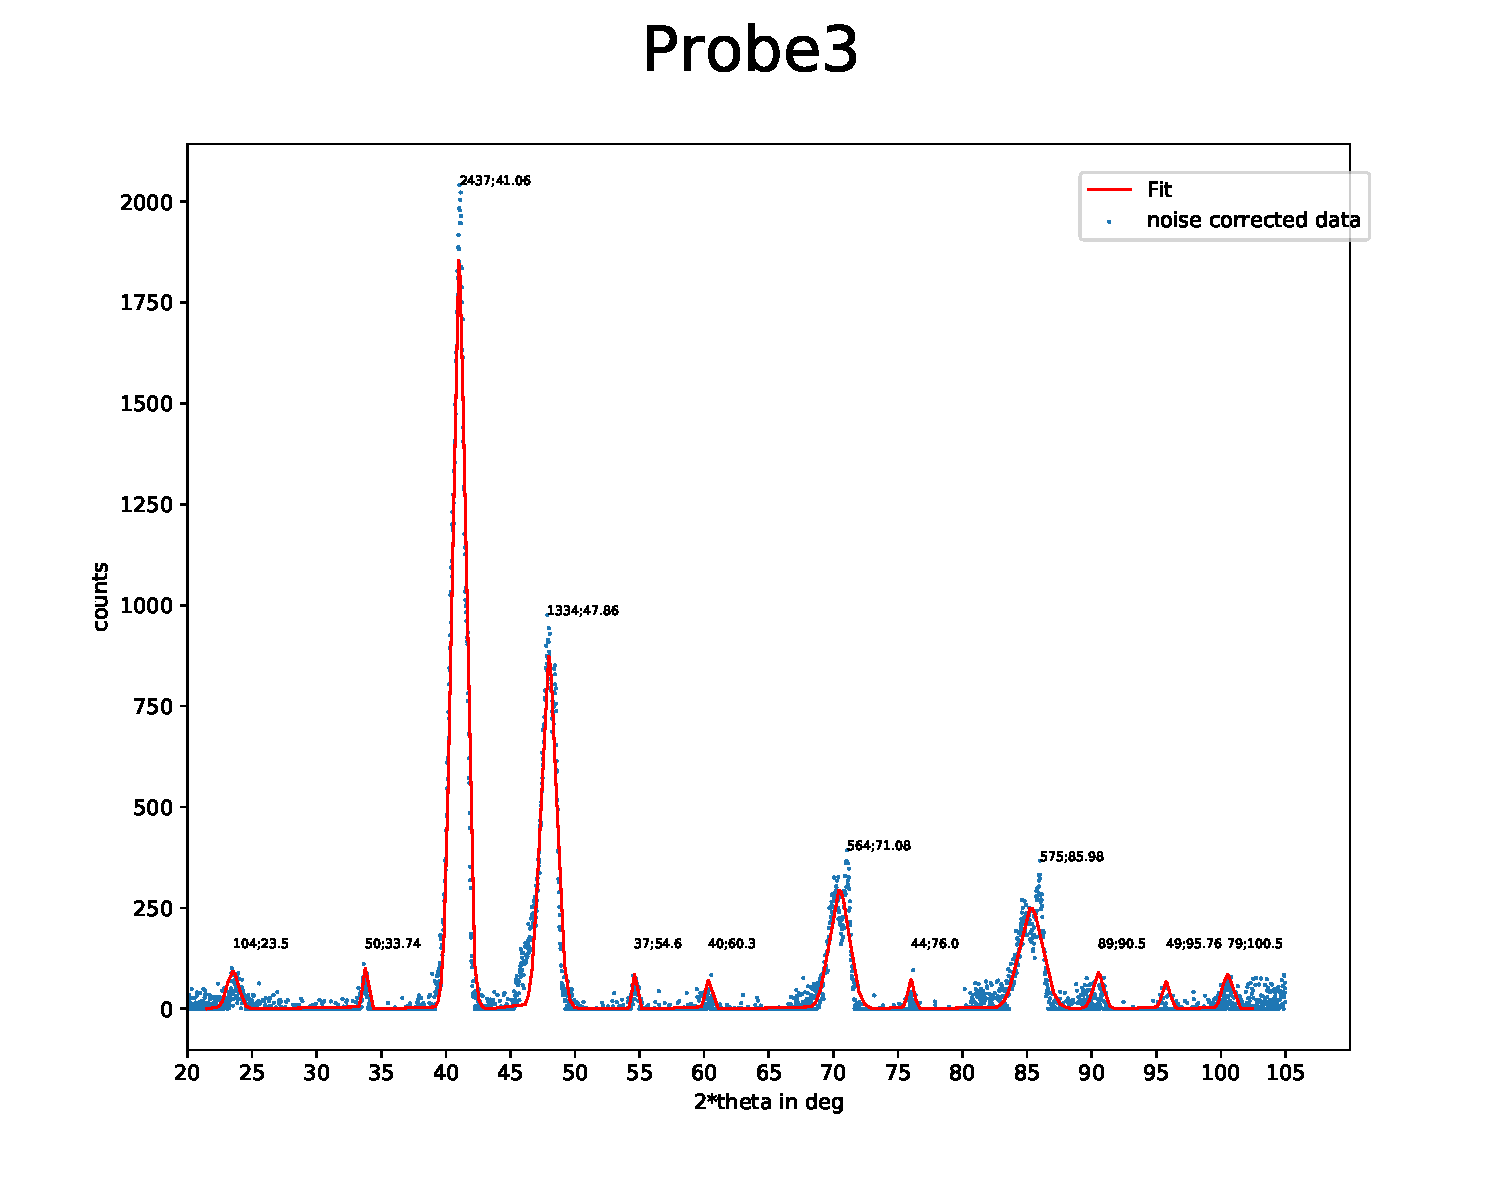
\includegraphics[width=0.8\textwidth]{Messdaten/Auswertungsskripte/Probe3.pdf}
        \caption{Röntgendiffraktogramm Probe 3}
        \label{Röntgendiffraktogramm Probe 3}
    \end{figure}
    \begin{figure}[H]
        \centering
        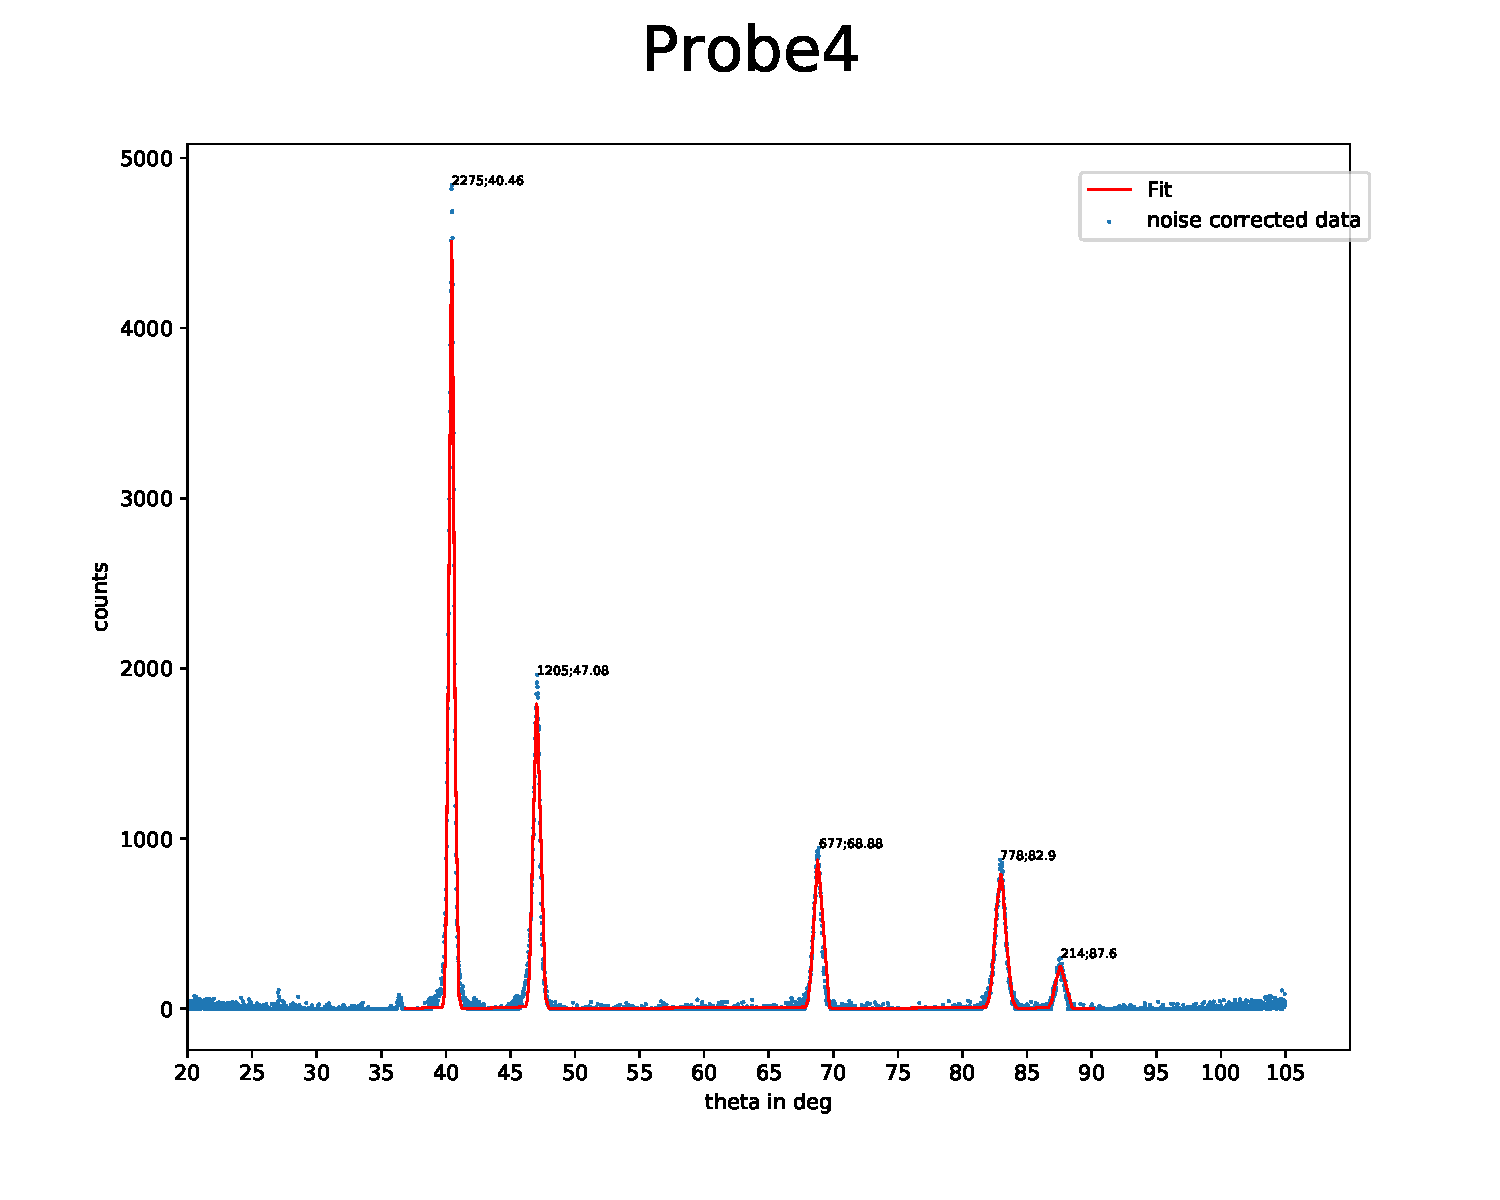
\includegraphics[width=0.8\textwidth]{Messdaten/Auswertungsskripte/Probe4.pdf}
        \caption{Röntgendiffraktogramm Probe 4}
        \label{Röntgendiffraktogramm Probe 4}
    \end{figure}

\begin{thebibliography}
    \bibitem[1]{https://docplayer.org/53918022-Versuchsanleitung-fuer-das-fortgeschrittenenpraktikum-ordnungseinstellung-in-cu3au-fp7-kilian-sinz.html}
\end{thebibliography}
